\documentclass[12pt,a4paper]{article}
\usepackage[utf8]{inputenc}
\usepackage[french]{babel}
\usepackage[T1]{fontenc}
\usepackage{mathtools}
\usepackage{amsfonts}
\usepackage{amssymb}
\usepackage[pdftex]{graphicx}
\usepackage{comment}
\usepackage[colorinlistoftodos,prependcaption,textsize=tiny]{todonotes}
\usepackage[left=2cm,right=2cm,top=2cm,bottom=2cm]{geometry}
\author{Angelo Ortiz}
\title{Rapport du Projet}

\begin{document}
\begin{titlepage}
  \centering
  
\includegraphics[width=0.30\textwidth]{logo.jpg}\par\vspace{1cm}
  {\scshape\LARGE Sorbonne Universit\'e\par}
  \vspace{1cm}
  {\scshape\Large 2I013 : Projet (application)\par}
  \vspace{1.5cm}
  {\Large \bfseries Sujet :\par}
  {\huge\bfseries IA Football\par}
  \vspace{2cm}
  {\Large\itshape Fangzhou Ye\par}
  {\Large\itshape Angelo Ortiz\par}
  \vfill
  
  % Bottom of the page
  {\large Licence d'Informatique\par}
  {\large Ann\'ee 2017/2018\par}
\end{titlepage}
 
%\newpage
\tableofcontents
  
\newpage
  
\part*{Introduction}
\section*{Pr\'esentation}
Le projet a consist\'e en le d\'eveloppement d'intelligences artificielles de 
joueurs de football. Le simulateur du jeu \'etant d\'ej\`a fourni, notre 
travail a \'et\'e d'impl\'ementer des strat\'egies de jeu pour mieux r\'eussir 
les matches.

L’objectif du travail a \'et\'e d'apprendre \`a bien mener un projet long 
sur un nouvel environnement de d\'eveloppement, \`a savoir 
Python. Sachant que travail \`a \'et\'e fait en bin\^ome, on a eu 
besoin d'un outil collaboratif, en l'occurrence {\bfseries git} qui est un 
logiciel de gestion de versions d\'ecentralis\'e. On a ainsi appris \`a g\'erer 
l'avancement d'un projet \`a travers la m\'ethode par fonctionnalit\'es.
\section*{Aper\c{c}u}
Voici un aper\c{c}u du simulateur de football lors d'une partie de notre 
\'equipe {\itshape ChPerFusion} en rouge face \`a l'\'equipe d'un de nos 
camarades de classe.

\begin{center}
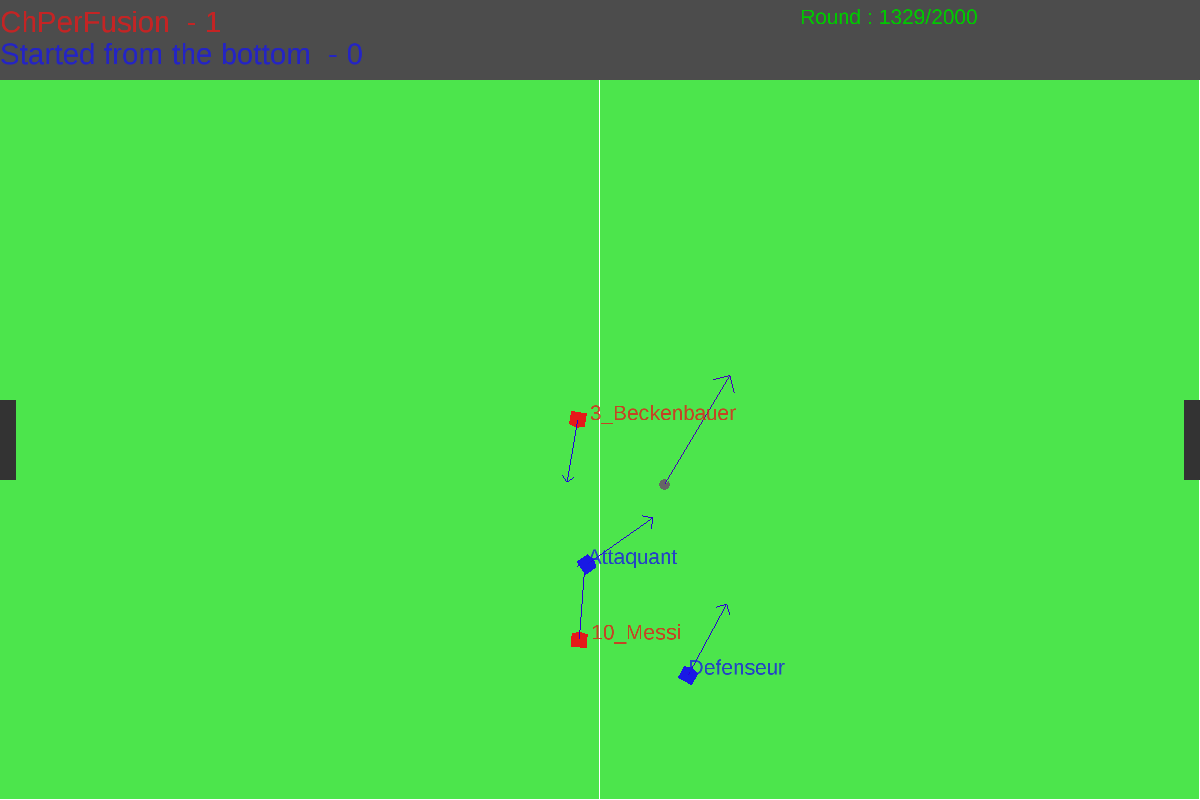
\includegraphics[width=0.8\textwidth]{apercu.png}\par%\vspace{1cm}
\end{center}

\section*{Diagrammes}
Le projet a \'et\'e organis\'e en un module {\bfseries ia} qui contient 
l'impl\'ementation nos joueurs et en divers fichiers de test.

On vous pr\'esente le graphe de d\'ependences du module.

\begin{center}
  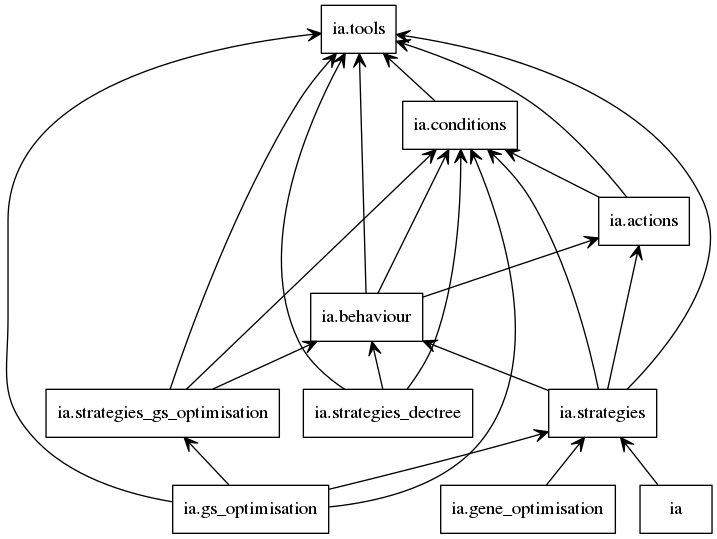
\includegraphics[width=0.8\textwidth]{packages_IA.png}\par%\vspace{1cm}
\end{center}

On vous pr\'esente \`a pr\'esent le diagramme de classes du projet.

\begin{center}
  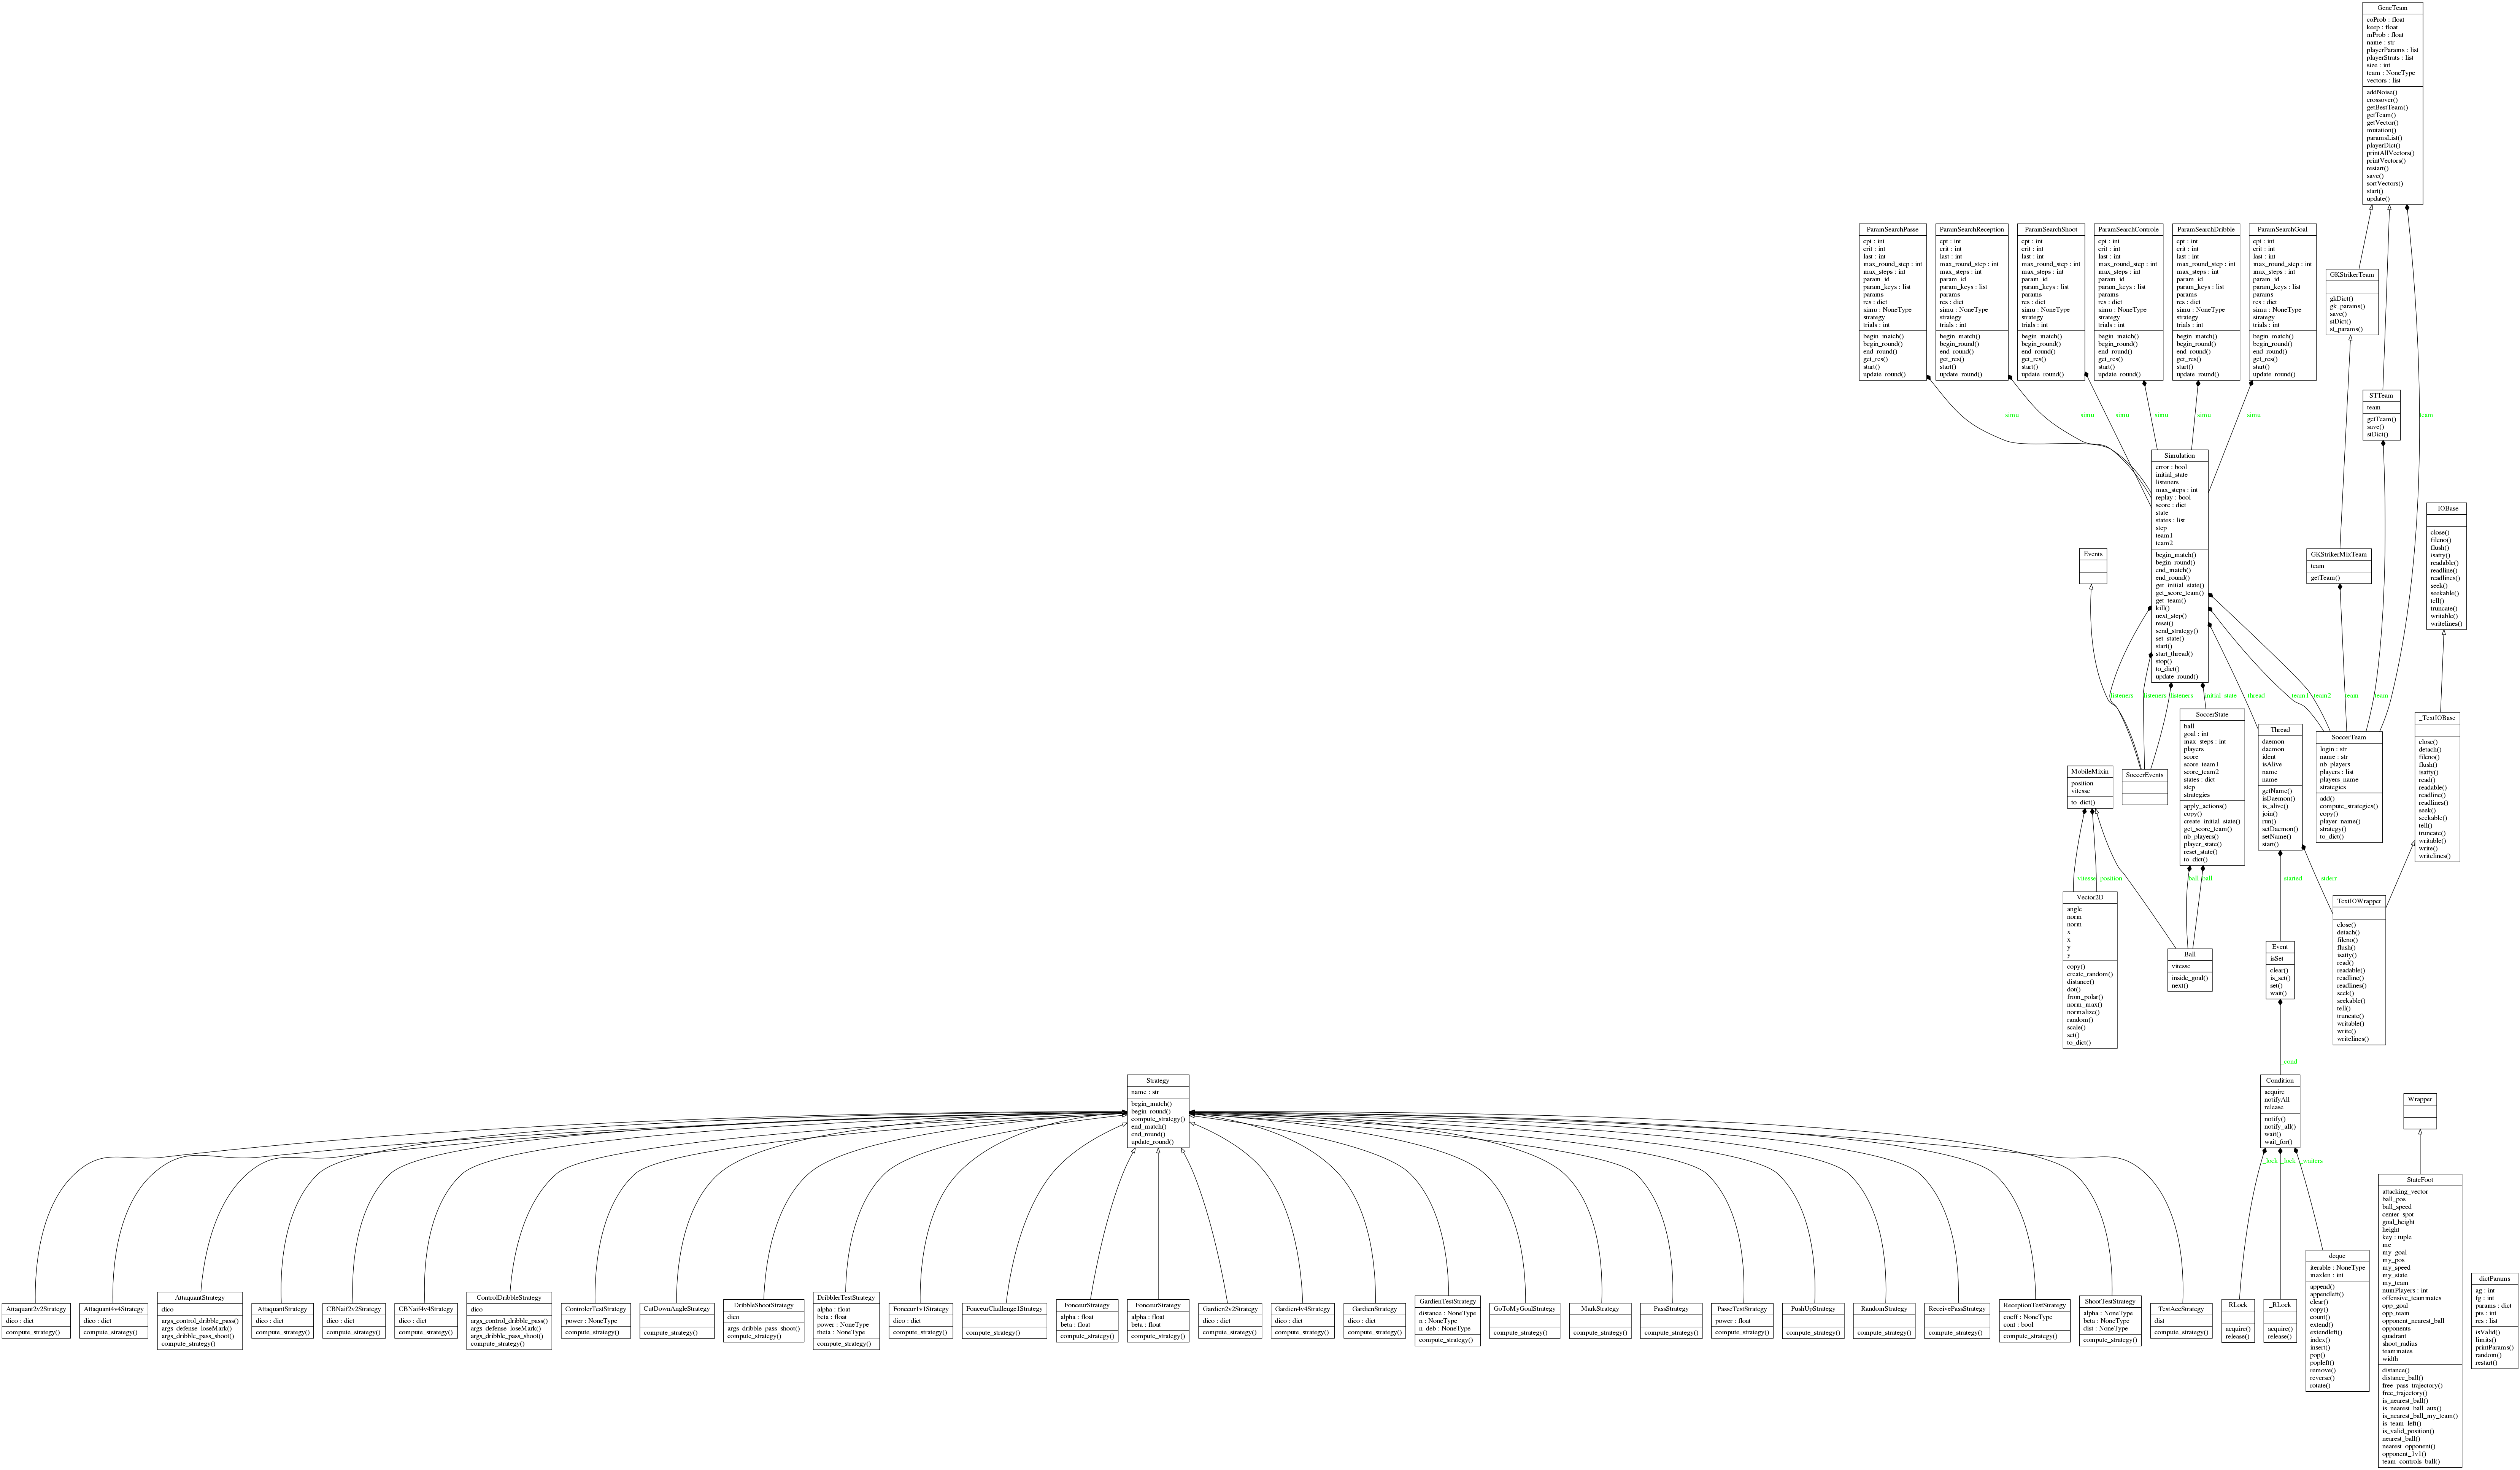
\includegraphics[width=0.8\textwidth]{classes_IA.png}\par%\vspace{1cm}
\end{center}


\addcontentsline{toc}{part}{Introduction}
\newpage

\part{Architecture logicielle} %et demarche
Dans cette premi\`ere partie, on vous expliquera les choix faits 
concernant l'architecture logicielle.

\newpage

\part{Strat\'egies}
Dans cette deuxi\`eme partie, on vous d\'etaille le comportement de nos 
diff\'erents joueurs.

Compte tenu de la taille du terrain de jeu, le nombre maximum de joueurs par 
\'equipe est limit\'e \`a quatre. Ainsi, il y a trois cat\'egories de matches 
selon le nombre de joueurs par \'equipe : un, deux ou quatre.

\section{Un joueur}
Pour l'\'equipe compos\'ee uniquement d'un joueur, on a d\'evelopp\'e un seul 
joueur que l'on appelle {\itshape Fonceur}. 

\subsection*{Fonceur}
Au tout d\'ebut du projet, il faisait tout au maximum : il doit 
s'approcher de la balle \`a toute vitesse lorsqu'il ne la contr\^ole pas et il 
frappe avec toute sa puissance dans le cas contraire. On a d\'ecid\'e de garder le 
m\^eme nom, m\^eme si son comportement diff\`ere. En effet, \`a pr\'esent il 
avance avec la balle de petites distances et lorsqu'un adversaire lui fait 
opposition il essaie de le dribbler ; il frappe vers la cage adverse s'il se 
trouve dans la surface de r\'eparation. 

\section{Deux joueurs}
Cette cat\'egorie a \'et\'e celle sur laquelle on a consacr\'e la plupart du 
projet. On compte trois jocusp pointueurs fonctionnels que l'on appelle 
{\itshape Attaquant}, {\itshape Gardien} et {\itshape D\'efenseur}. 

\subsection*{Attaquant}
Il a une vocation plut\^ot offensive. Il se comporte diff\'eremment selon 
s'il contr\^ole la balle ou pas. Dans la premi\`ere situation, il essaie 
syst\'ematiquement d'avancer sur le terrain balle au pied et de faire un tir 
vers la cage d\`es qu'il se trouve dans la surface de r\'eparation adverse. 
Cependant, s'il rencontre un adversaire lui bloquant le chemin, il tente de 
faire une passe vers son co\'equipier s'il est sans marquage, il le 
dribble sinon. 

Il montre trois conduites lorsqu'il se trouve sans le 
contr\^ole du ballon : il presse le porteur de la balle s'il en plus 
proche que son co\'equipier, il se d\'ecale lat\'eralement dans le cas 
contraire, et il monte dans le terrain si c'est son co\'equipier qui la 
poss\`ede ou va bient\^ot en prendre possession pour lui proposer une 
possiblit\'e de passe.

\subsection*{Gardien}
De la m\^eme mani\`ere que pour le fonceur, le gardien ne garde gu\`ere de son 
comportement initial. Il restait fix\'e dans sa cage et en sortait juste pour 
r\'eduire l'angle de frappe \`a l'attaquant adverse. Sa possession de la balle 
se r\'eduisait \`a un d\'egagement presque al\'eatoire.

On a remplac\'e sa conduite avec la balle par celle de l'attaquant 
mentionn\'e ci-dessus. En revanche, en absence du ballon, il reste \`a une 
distance de sa cage lorsque l'\'equipe adverse le contr\^ole et essaie 
de l'intercepter lorsque le porteur se trouve dans sa surface de r\'eparation. 
Tout comme pour l'attaquant, il monte dans le terrain lorsque n\'ecessaire.

\subsection*{D\'efenseur}
Le d\'efenseur n'a par contre qu'une vocation d\'efensive. En effet, s'il a la 
balle, il s'en d\'efait le plus rapidement possible soit \`a l'aide d'une passe 
vers son co\'equipier si d\'emarqu\'e, soit via le d\'egagement le moins 
risqu\'e possible. Quant \`a son effort d\'efensif, il demeure \`a une certaine 
distance radial \`a partir de sa cage et s'approche de la balle en vu d'une 
interception s'il en suffisamment proche.

\section{Quatre joueurs}
Il s'agit de la cat\'egorie que l'on a trouv\'e la plus int\'eressante en 
raison de la difficult\'e de la gestion des espaces et la r\'epartition des 
fonctions. Tout comme pour la cat\'egorie pr\'ecedente, on compte trois 
joueurs fonctionnels que l'on rep\`ere d'ailleurs par les m\^emes noms. 

\subsection*{Attaquant}
Il y a deux diff\'erences en son comportement par rapport \`a son pair 
de la cat\'egorie ci-dessus et celles-ci concernent toutes les deux la 
situation o\`u il se trouve dans sa surface de r\'eparation. La premi\`ere fait 
r\'ef\'erence \`a la r\'ecup\'eration de la balle : il ne se 
pr\'ecipite plus et se comporte tel qu'il le fait dans le milieu du terrain. La 
deuxi\`eme correspond \`a l'effort de marquer les adversaires sans 
marquage.

\subsection*{Gardien}
Ce joueur combine le comportement de son pair de la cat\'egorie ci-dessus et de 
l'attaquant de cette cat\'egorie. En effet, il suit les m\^emes indications que 
l'attaquant lorsqu'il contr\^ole et r\'ealise les m\^emes mouvements sans ballon 
que le d\'efenseur de l'\'equipe \`a deux joueurs.

\subsection*{D\'efenseur}
Ce d\'efenseur prend les m\^emes d\'ecisions que celui de l'\'equipe \`a 
deux joueurs, \`a l'exception de sa prise de risque lors d'une interception. 
Effectivement, si un co\'equipier se trouve dans une meilleure position pour 
intercepter la balle, i.e.\ il en est plus proche que le d\'efenseur, celui-ci 
continue de positionner radialement \`a une certaine distance de sa cage.

\newpage

\part{M\'ethodes d'optimisation}
Dans cette troisi\`eme partie, on vous d\'etaille les diff\'erents algorithmes 
appris tout au long du semestre pour l'am\'elioration des strat\'egies 
initialement propos\'ees.

\section{Recherche en grille}
La premi\`ere m\'ethode d'optimisation pre\'esent\'ee en cours a \'et\'e la 
recherche en grille. Celle-ci est utilis\'ee pour l'optimisation d'une 
action.

Tout d'abord, on doit d\'efinir l'action \`a optimiser et le crit\`ere 
d'optimalit\'e, et rep\'erer les param\`etres associ\'es. Puis on 
obtient un ensemble de valeurs pour chaque param\`etre. 
Pour les param\`etres discrets, il suffit de prendre toutes les valeurs 
possibles, alors que pour les param\`etres continus il faudra faire en amont 
une discr\'etisation, i.e.\ on divise l'intervalle d\'elimit\'e par des bornes 
d\'efinies selon un pas de pr\'ecision. On compte ainsi des vecteurs dont les 
coordonn\'ees correspondent chacune \`a un param\`etre. On fait ensuite une 
recherche exhaustive sur tous les vecteurs obtenus : on teste chaque vecteur 
sous diff\'erents conditions environnementales et on moyenne les \'evaluations 
 du crit\`ere dans lesdites conditions. Finalement, on prend la valeur optimale 
et son vecteur associ\'e.

Il est important de remarquer que la plupart de nos param\`etres sont continus. 
Pour obtenir des valeurs plus pr\'ecises et un meilleur comportement, on a 
besoin d'un pas de discr\'etisation tr\`es petit. Ainsi, on r\'ealise qu'une 
augmentation du nombre de param\`etres \`a optimiser a une tr\`es forte 
influence sur le temps d'ex\'ecution de l'algorithme mis en place. On en 
d\'eduit que le minuscule gain relatif nombre de param\`etres--temps 
d'ex\'ecution ne convient pas au moyen terme.

\section{Algorithmes g\'en\'etiques}
Dans un deuxi\`eme temps, on est pass\'es aux algorithmes g\'en\'etiques. On en 
a mis en place une impl\'ementation pour optimiser les \'equipes compos\'ees 
d'un ou deux joueurs.

Cette classe d'algorithmes se base sur la th\'eorie de l'\'evolution. En effet, 
la notion de s\'election naturelle est le m\'ecanisme permettant de choisir des 
solutions potentielles de plus en plus meilleures.

La toute premi\`ere chose \`a faire est la d\'efinition de la fonction 
$f: \mathbb{R}^n \to \mathbb{E}$ \`a optimiser, o\`u $n$ est le nombre de 
param\`etres concern\'es. Un \'el\'ement $x=(x_1,\dotsc,x_n) \in \mathbb{R}^n$ 
est appel\'e {\itshape candidat} ou {\itshape chromosome}, et chacune de ses 
coordonn\'ees $x_i$ avec $i=1,\dotsc,n$, appel\'ee {\itshape propri\'et\'e} 
ou encore {\itshape g\`ene}, correspond \`a un param\`etre \`a optimiser. Elles 
forment le {\itshape g\'enotype}.
Autrement dit, un candidat correspond \`a une \'equipe d\'efinie par les valeurs
de ses propri\'et\'es.

Dans le cadre du projet, on a d\'efini $f(x)=(V,N,D,P,C)$ comme le 
bilan apr\`es avoir disput\'e plusieurs matches avec les m\^emes valeurs des 
param\`etres donn\'ees par $x$, i.e.\ le tuple compos\'e du 
nombre de 
victoires, matches nuls, d\'efaites, buts marqu\'es et buts encaiss\'es. La 
relation d'ordre suit les r\`egles du classement d'un tournoi de football.

Cette classe d'algorithmes comportent quatre \'etapes.

\begin{enumerate}
\item \underline{Initialisation :} Tout d'abord, il faut g\'en\'erer un 
ensemble de candidats $\{x_1,\dotsc,x_m\}$. Le but est d'obtenir une population 
initiale la plus diverse possible de sorte \`a pouvoir atteindre le plus de 
maxima relatifs. C'est pourquoi cette premi\`ere g\'en\'eration est obtenue de 
mani\`ere al\'eatoire.
\item \underline{\'Evaluation :} Ensuite, on \'evalue la fonction en 
chacun des candidats, i.e.\ on calcule $\{f(x_1),\dotsc,f(x_m)\}$.
\item \underline{S\'election :} Suivant la notion de s\'election 
naturelle, on ne conserve que les candidats avec les meilleurs r\'esultats. 
Autrement dit, on dresse un classement des \'equipes associ\'ees aux candidats 
et n'en garde qu'une partie.
\item \underline{Reproduction :} Finalement, on attribue les places 
libres aux candidats n\'es du brassage g\'en\'etique des candidats les 
plus performants. Pour ce faire, on compte sur deux m\'ethodes, \`a savoir le 
croisement et la mutation. \'Etant donn\'e deux parents, on commence par les 
cloner en deux enfants. Puis on choisit une ligne de coupe divisant le 
g\'enotype en deux parties. Ensuite, les enfants s'\'echangent une partie de 
leur g\'enotype. Le croisement s'arr\^ete \`a ce stade-l\`a, tandis que la 
mutation ajoute du bruit al\'eatoirement dans un g\`ene pour chacun 
des nouveaux chromosomes. On a d\'ecid\'e de faire une petite modification \`a 
cette \'etape-l\`a lors de l'impl\'ementation pour avoir plus de 
diversification : une minorit\'e des places libres est attrribu\'ee \`a des 
candidats g\'en\'er\'es al\'eatoirement.
\end{enumerate}

Cet algorithme \'etant it\'eratif, on recommence \`a la deuxi\`eme phase avec 
la nouvelle g\'en\'eration. Au bout d'un nombre raisonnable d'it\'erations, on 
se retrouve avec une g\'en\'eration compos\'ee de chromosomes tr\`es proches des 
maxima relatifs. On finit donc l'algorthme par prendre le candidat optimal de la 
derni\`ere population.  

\section{Apprentissage automatique}
Dans la derni\`ere partie du semestre, on s'est concentr\'e sur l'apprentissage 
automatique. On nous a pr\'esent\'e les deux grandes familles 
d'algorithmes d'apprentissage : supervis\'es et non supervis\'es, ainsi que 
l'apprentissage par renforcement. Deux m\'ethodes ont \'et\'e impl\'ement\'ees 
lors du projet.

\subsection*{Arbres de d\'ecision (de classification)}
Il s'agit d'une technique d'apprentissage supervis\'e. Pour l'appliquer, on 
a besoin d'un espace de repr\'esentation $\mathcal{X}$, d'un ensemble 
d'\'etiquettes ou classes $Y$ et d'une liste de $m$ exemples d'apprentissage 
$(x^i,y^i)$, o\`u $x^i \in \mathcal{X}$, $y^i \in Y, i = 1,\dotsc,m$, appel\'ee 
ensemble d'apprentissage.
Le but de cette technique est de trouver une fonction $f: \mathcal{X} \to 
Y$ telle que l'on puisse pr\'edire \`a quelle classe appartient une 
future variable $x \in \mathcal{X}$.

Concr\`etement, on veut associer une certaine action \`a chaque \'etat du jeu. 
Comme le nombre d'\'etats possibles est trop grand, on utilisera une 
repr\'esentation par $n$ caract\'eristiques g\'en\'eralis\'ees qui 
pr\'ecisent la configuration du terrain. On a ainsi que $\mathcal{X} = 
\mathbb{R}^n$, avec $n$ la dimension de l'espace de repr\'esentation. De plus, 
l'ensemble d'\'etiquettes devient l'ensemble d'actions possibles $A$. On veut 
donc trouver une fonction $f: \mathbb{R}^n \to A$ qui fournit la meilleure 
action possible pour tout \'etat du jeu.

Le probl\`eme auquel on est confront\'es se r\'eduit alors \`a 
partitionner l'espace de repr\'esentation en $p=|A|$ parties 
$\mathcal{X}_1,\mathcal{X}_2,\dotsc,\mathcal{X}_p$ de sorte que 
$f([\mathcal{X}_i]) = \{ a_i \} \subset A$, $i = 1,\dotsc,p$. On utilise les 
arbres de d\'ecisions pour repr\'esenter ce partionnement. Ceci 
implique que chaque n\oe ud interne correspond \`a un test sur une des $n$ 
dimensions de $\mathcal{X}$, chaque feuille correspond \`a l'action \`a 
entreprendre pour l'\'etat donn\'e par le chemin suivi depuis la racine.

\subsection*{Q-learning}
Cet algorithme d'apprentissage par renforcement r\'epose sur un ensemble 
d'\'etats $S$, un ensemble d'actions $A$, et une fonction $Q: S \times A \to 
\mathbb{R}$, appel\'ee {\itshape politique}, pond\'erant une paire form\'ee 
par un {\itshape \'etat} donn\'e et une action \`a entreprendre pour cet 
\'etat-ci. Cette pond\'eration est surnomm\'ee {\itshape r\'ecompense}. La 
notion d'\'etat correspond \`a celle donn\'ee dans la section des arbres 
binaires. Il utilise aussi la notion d'{\itshape \'episode} que l'on associe 
\`a un match dans le cadre du projet. Son principe est le suivant : on apprend 
une politique comportementale qui optimise l'esp\'erance des r\'ecompenses.

La premi\`ere phase consiste \`a initialiser $Q$ \`a une valeur fixe 
arbitraire, ici 0. La deuxi\`eme phase concerne un \'episode, ou encore un 
match, et est r\'ep\'et\'ee autant de fois qu'il y a d'\'episodes. Pour un 
\'etat $s_t$ donn\'e, on choisit une action $a_t$ selon la politique $Q$ et 
observe la r\'ecompense $r_t$ associ\'ee \`a cette paire. Cette action 
g\'en\`ere un nouvel \'etat $s_{t+1}$. Il est \`a noter qu'il n'y a pas de 
choix concernant l'\'etat initial $s_0$, puisqu'il est toujours le m\^eme pour 
un match de football : ceci correspond au coup d'envoi. Ensuite, on met \`a 
jour la politique selon la formule ci-dessous.

\begin{equation*}
  Q(s_t,a_t) \gets (1-\alpha) \cdot 
  \underbrace{Q(s_t,a_t)}_{\mathclap{\text{valeur actuelle}}} + \ \alpha \cdot 
\underbrace{\Big(r_t + \gamma \cdot \max_a(Q_{t+1},a) 
  \Big)}_{\mathclap{\text{valeur   apprise}}}
\end{equation*}

Ici, $\alpha$ repr\'esente la vitesse d'apprentissage et $\gamma$ le facteur 
d'actualisation. D'un c\^ot\'e, la vitesse d'apprentissage d\'etermine 
l'\'equilibre entre exploration et exploitation. En effet, une valeur de 
0 implique l'utilisation exclusive des choix actuels, alors qu'une 
valeur 1 ne ferait que consid\'erer le dernier r\'esultat.
D'un autre c\^ot\'e, le facteur d'actualisation d\'etermine l'importance des 
r\'ecompenses futures. Une valeur de 0 ne prend en consid\'eration que les 
r\'ecompenses courantes, tandis qu'une valeur de 1 met en valeur les 
r\'ecompenses plus lointaines. On avait pr\'ecis\'e qu'un \'episode 
correspondait \`a un match ; par cons\'equent, la r\'eussite d'une succession 
d'actions d\'epend du r\'esultat final du match. De ce fait, on a int\'er\^et 
\`a retarder au maximum les r\'ecompenses. Ceci se traduit par le choix d'un 
facteur $\gamma$ proche de 1.

Juste apr\`es la mise \`a jour de la politique $Q$, on d\'etermine si l'\'etat 
$s_t$ est terminal, i.e.\ qu'il correspond au coup de sifflet final. Dans le 
cas affirmatif, on passe \`a l'\'episode suivant ou on s'arr\^ete selon s'il y 
en a encore \`a faire, alors que l'on r\'eit\`ere cette phase \`a partir du 
choix d'une action pour le nouvel \'etat $s_{t+1}$ dans le cas contraire.

\`A la fin de l'algorithme, on se retrouve avec une politique qui nous rend 
l'action la plus ad\'equate pour tout \'etat du jeu. \'Etant donn\'e que les 
carat\'eristiques utilis\'ees pour d\'efinir un \'etat sont continues, 
on a d\'efini des intervalles d'\'equivalence. Cela n'emp\^eche que le nombre 
total d'\'etats est \'enorme et fait donc exploser la m\'emoire. On pourrait 
mettre en place un r\'eseau de neurones pour pallier cette difficult\'e. Ceci 
n'a pas \'et\'e le cas pour ce projet et donc, bien qu'impl\'ement\'e, on 
s'est pas servi de cet algorithme pour am\'eliorer nos strat\'egies. 

\newpage

\part*{Conclusion}
...
\addcontentsline{toc}{part}{Conclusion}

\end{document}
